
\documentclass[fontsize=9pt]{scrartcl}
\usepackage{custom}


\title{{'{'}}{{cookiecutter.description}}{{'}'}}


\author[1]{ {{cookiecutter.author_name}}\thanks{ {{cookiecutter.email}} } }
% \author[1,2]{Random Name\thanks{r.name@uni.co.uk}}
% \affil[1]{School of Electronics Engineering and Computer Science, Queen Mary, University of London, London E1 4NS, United Kingdom}
\affil[1]{School of things, University of stuff, City XXXXX, Country}
% \affil[2]{Company, City XXXXX, Country}


\addbibresource{{'{'}}{{cookiecutter.repo_name}}.bib}

\begin{document}

\maketitle

\begin{abstract}
\lipsum[1]
\end{abstract}

\begin{multicols}{2}


\lipsum[2]

\section{First section}


\subsection{First subsection}

Testing \textbf{bold}, \textit{italics}, \textit{\textbf{bold italics}}.
Trying $a^3$

\lipsum
Let us try to cite this article \cite{knuth:ct:a}, which is really good. Also
there is things on \fig{fig:1}. \\
Here is some math:

\begin{equation}
B'=-\nabla \times E
\end{equation}


\begin{figure}[H]
  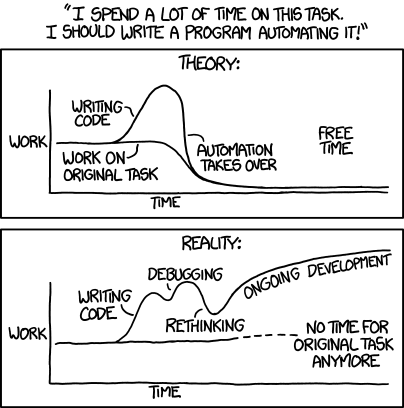
\includegraphics[width=1\columnwidth]{img}
  \caption{Quisque ullamcorper placerat ipsum. Cras nibh. Morbi
vel justo vitae lacus tincidunt ultrices. Lorem ipsum dolor
 sit amet, consectetuer adipiscing elit. In hac habitasse
platea dictumst. Integer tempus convallis augue. Etiam facilisis.}
  \label{fig:1}
\end{figure}



\begin{table}[H]
\centering
 \begin{tabular}{||c c c c||}
 \hline
 Col1 & Col2 & Col2 & Col3 \\ [0.5ex]
 \hline\hline
 1 & 6 & 87837 & 787 \\
 2 & 7 & 78 & 5415 \\
 3 & 545 & 778 & 7507 \\
 4 & 545 & 18744 & 7560 \\
 5 & 88 & 788 & 6344 \\ [1ex]
 \hline
 \end{tabular}
 \caption{Lacus tincidunt ultrices. Lorem ipsum dolor
  sit amet, consectetuer adipiscing elit.}
\end{table}



\lipsum[2-6]
\vspace*{1em}

\printbibliography[title=References]
%


\end{multicols}


\end{document}
